\section{Implementierung}
\label{sec:implementierung}

\todo{Einleitungssatz}%

\subsection{Client - Darstellung}
\label{subsec04:client_viz}

\todo{Einleitungssatz}%

\subsubsection{Informationen vom Server}
\label{subsubsec04:info_server}

In der schon bereits vorhandenen Software gibt es eine erste Implementierung, die die Informationen vom Server an den Client sendet.
Der Client speichert dies Informationen in einem ``Interface'' (siehe: Listing~\ref{lst:desc_schema}). 

\lstinputlisting[
  language=javascript,
  caption=Interface einer Tabelle und Spalte,
  label=lst:desc_schema,
  float=h,
  numbers=left
]{snippets/schema.description.ts}

Eines der Grundprinzipien von Typescript ist die Typprüfung. Interfaces erfüllen dabei die Rolle der Benennung der Typen und bestimmen Schnittstellen innerhalb des Projektes und zum Code ausserhalb.~\cite{typescript_interfaces}

Damit ist festgeschrieben welche Eigenschaften eine Tabelle und die dazugehörigen Spalten besitzen müssen. Bis zu diesem Zeipunkt wurden die Informationen der Datenbank, nur verwendet diese Anzuzeigen. Mit der dazu kommenden Funktionalität der Migration, werden Funktionen auf einzelne Tabellen oder Spalten angewendet. Diese Funktionen lassen sich nicht in einem Interface abspeichern. Für eine leichtere Anwendung und der Verhinderung globale Funktionen zu definieren wurden zwei Klassen implmentiert. In einer Tabellen und Spalten Klasse konnten dann die einzelnen Funktionen für die weitere Implementierung programmiert werden.


\subsubsection{Fehlende Foreign Keys}
\label{subsubsec04:miss_fk}

Bei der Analyse der Daten die vom Server versendet werden (siehe: Listing~\ref{lst:desc_schema}), wurde festgestellt, dass die Foreign Keys der einzelnen Tabellen nicht übermittelt wurden.
Für die akurate Darstellung des Schemas sind die Foreign Keys der einzelnen Tabellen notwendig, um die einzelnen Relationen anzeigen zu können.
Dafür mussten die Informationen zuerst von der Datenbank erfragt und dann versendet werden (siehe dafür:~\ref{subsubsec04:fk_table_server}).
Da im Gegensatz zu Tabellen und Spalten keine direkten Veränderungen an Foreign Keys möglich sind, sondern nur das Hinzufügen und Entfernen dieser, müssen diese nicht in einer eigenen Klasse abgebildet werden.

\lstinputlisting[
  language=javascript,
  caption=Interface: Foreign Keys,
  label=lst:fk,
  float=h,
  numbers=left
]{snippets/foreign_key.description.ts}

\subsubsection{Anzeige des Schemas}
\label{subsubsec04:anz_schema}

Die Darstellung des Schemas ist der Einstiegspunkt der Komponente und soll neben der Darstellung auch die Bedienung und weiterleitung zu den weiteren Funktionen liefern.

\begin{description}
\item[Angular 2] \hfill\\
Im ersten Schritt wurden die Daten, die vom Server zur Verfügung gestellt wurden in simpler Art auf dem Bildschirm dargestellt. 
Dafür bietet Angular 2 ``Templates'' an. Templates definiert damit das Aussehen einer Komponente. Templates sehen dabei aus wie \texttt{HTML}-Dokumente, mit ein paar Unterschieden~\cite{angular2_flow}.

\begin{figure}[ht]
    \frame{\includegraphics[width=\textwidth]{images/kap-4-angular2_overview.png}}
    \centering
    \caption{Angular 2 Architectur}
    \label{pic:angular2_architecture}
\end{figure}

Bei diesen Unterschieden handelt es sich um Erweiterungen, die bestimme Funktionalitäten zu dem \texttt{HTML} Standart hinzufügen. Die wichtigsten und in diesem Projekt am häufigsten angewandten Erweiterungen sind folgende:
\begin{itemize}
\item Variablen aus einer Komponente direkt zu zugreifen (Property Binding)
\item Funktionen direkt an Events zu verknüpfen (Event Binding)
\item If-Anweisungen 
\item Schleifen
\end{itemize} 


\item[Bootstrap] \hfill\\
Bootstrap ist ein \texttt{CSS}-Framework, welches in dem Projekt bereits eingebunden ist. Damit lassen sich auf schnelle und einfache Art \texttt{HTML}-Dokumente gestalten. 
Eines der in Bootstrap vorhandenen Gestaltungsvorlagen sind die ``Cards''\footnote{\url{https://v4-alpha.getbootstrap.com/components/card/}} die für die Gestaltung der einzelnen Tabellen benutzt wurde.

\begin{figure}[ht]
    \frame{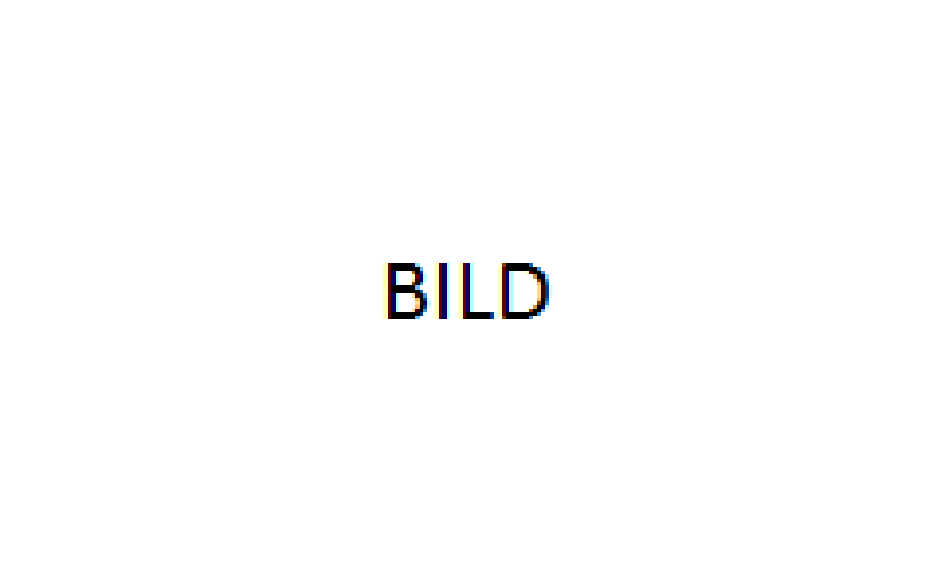
\includegraphics[width=\textwidth]{images/dummy.png}}
    \centering
    \caption{Darstellung einer Tabelle mit Bootstrap}
    \label{pic:table_boot}
\end{figure}

\item[Font Awesome] \hfill\\
Um die Darstellung ein wenig angenehmer für die Benutzer zu machen, wurde auf ein Symbole zurückgegriffen um einige Informationen in der Tabelle oder Buttons darzustellen. In der urpsrünglichen Entwicklung der Software, wurde dafür der Icon-Font\footnote{\url{https://de.wikipedia.org/wiki/Font_(Informationstechnik)}} ``Font Awesome'' eingebunden. Dieser Font wurde unter anderem dann auch zur Visuallisierung der Primärschlüssels verwendet.(siehe: Grafik~\ref{pic:table_boot})\todo[color=green!40]{Bild hinzufügen}% 

\item[Graphviz] \hfill\\
Im bereits vorhandenen Server war eine Schnittstelle zu einem Graphviz-Service\footnote{\url{http://www.graphviz.org/}} integriert. Graphviz ist ein Programmpacket um Grafiken darzustellen. Dies konnte dazu verwendet werden eine Darstellung des Datenbankschemas zu erzeugen und anzuzeigen, als eine weitere Möglichkeit das ganze Schema auf einen Blick zu sehen, mit nur den nötigsten Informationen.
Ein Beispiel ist in der Grafik~\ref{pic:graphviz_schema} zu sehen.

\begin{figure}[ht]
    \frame{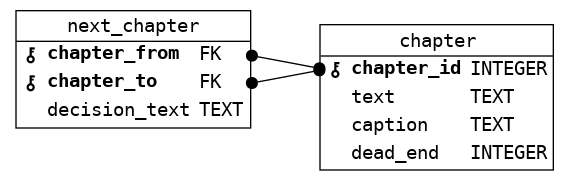
\includegraphics[width=\textwidth]{images/visual_schema.png}}
    \centering
    \caption{Graphviz Schema Darstellung}
    \label{pic:graphviz_schema}
\end{figure}

\item[Zusätzliche Darstellung der Foreign Keys] \hfill\\
\todo[inline]{Je nach der Darstellung der Foreignkeys}


\end{description}

\subsubsection{Tablleninhalte}
\label{subsubsec04:table_content}

In Blattwekzeug bestand bereits die Möglichkeit SQL-Statements auszuführen. Es ist also möglich eine Abfrage der Art ``\texttt{Select * from \textsc{Tabellenname}}'' auszuführen, und sich alle Daten aus einer Tabelle anzeigen zu lassen. In Anbetracht, dass Blattwekzeug eine Software ist, die zum erlenen von Datenbanken und deren Umgang dienen soll und zusätzlich auch viele ähnliche Programnme~\ref{sec02:vergleichbare_arbeiten} dies zur Verfügung stellen, soll es möglich sein, die Daten einer Tabelle in einer übersichtlichen Ansicht anzeigen zu lassen.
Die Daten kommen vom Server in einem 2-Dimensionalen Array, eine Dimension für jede vorhandene Spalte und die zweite Dimension für die einzelnen Zeilen der Spalte.
Im Detail wie die Daten im Server von der Datenbank abgefragt werden, wird hier~\ref{subsubsec04:anfragen_darstellung} 
besprochen.

Ein Beispiel einer solcher Darstellung ist in der Grafik dargestellt.

\begin{figure}[ht]
    \frame{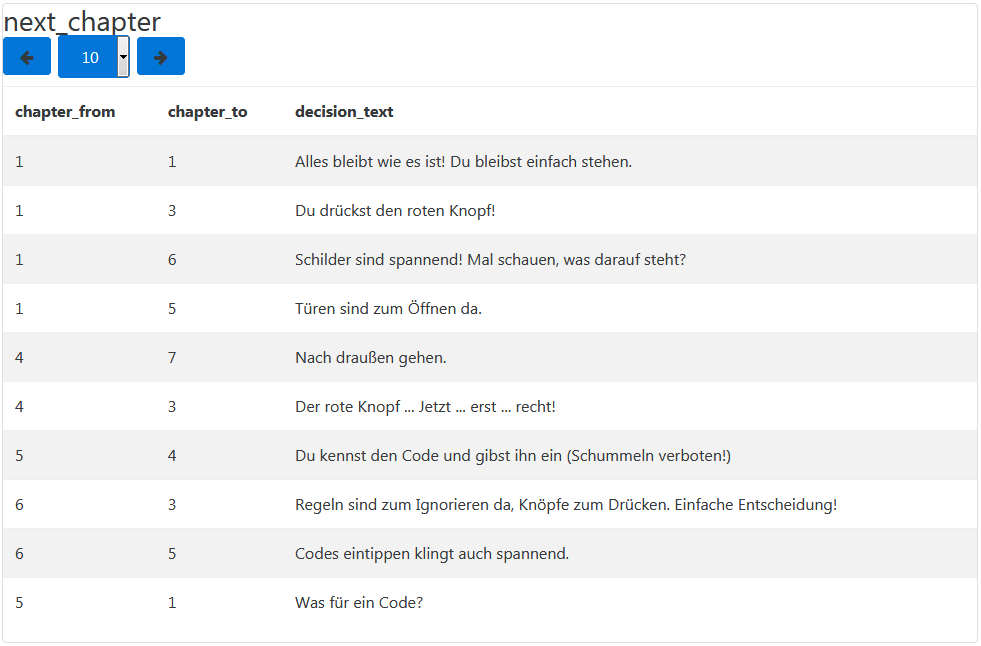
\includegraphics[width=\textwidth]{images/table_content.png}}
    \centering
    \caption{Darstellung der Tabelleninhalte}
    \label{pic:table_content}
\end{figure}

\begin{description}
\item[Verwendung Angular 2 \& Bootstrap] \hfill\\
In der Darstellung der Daten konnte das 2-Dimensionale Array direkt in dem Template der Komponente eingebunden werden. In folgenden sieht man die Verwendung der Angular 2 Templates mit der zusätzlichen Verwendung von Bootstrap, die im Abschnitt~\ref{subsubsec04:anz_schema} erwähnt wurden.
Dabei ist in Zeile 1 die \texttt{class}-Eigenschaft auf ``table table-striped'' gesetzt um die von Bootstrap zur Verfügung gestellte Tabellendarstellung zu verwenden. Dabei sorgt die zweite \texttt{class}-Eigenschaft, dass die Tabellenzeilen, zur besseren Übersicht, gestreift angezeigt werden.
In den Zeilen 5,13,14 sind die von Angular 2 Schleifen zu sehen und in Zeile 6 und 15, dass ``Property Binding'' wird auf eine Variable direkt aus der ``Component'' zugegriffen.

\lstinputlisting[
  language=HTML,
  caption=Code zur Darstellung von Tabelleninhalte,
  label=lst:fk,
  float=h,
  numbers=left
]{snippets/table_content.ts}

\item[Pagening] \hfill\\
Es ist zu berücksichtigen, dass einige Tabellen gefüllt sein können mit einer großen Menge an Daten. Damit ein endlos langes Scrollen verhindert wird, wurde ein ``Pagening'' eingebaut. Damit kann die Anzahl an angezeigten Daten gewählt werden, und mit den Pfeil-Buttons kann zwischen den Pages~\footnote{Seiten - Satz an Daten} angezeigt werden. 

\end{description}

\newpage

\subsection{Client - Editor}
\label{subsec04:client_edit}

Im folgenden Kapitel soll die Implementierung des Editors auf Clientsseite erklärt werden. Dieser und der korespondierende Serverseitige Abschnitt werden deutlich ausführlich behandelt, da es der Kern dieser Ausarbeitung ist.
Die Migration eines Schemas einder Datenbank, ist im Allgemeinen das Verändern der Datenbank, mit der Absicht diese auf neue Gegebenheiten anzupassen oder erweitern. Zusätzlich ist im allgemeinen Sinne der Migration, auch die Möglichkeit das Schema auf eine ältere Version zurückzuführen.
In Anbetracht der hier vorliegenden Software, wird nur die Möglichkeit geboten das Schema anzupassen ohne einer Versionskontrolle.
Da die Thematik der Schema Migration ein sehr komplexes ist, mit möglichen ir­re­ver­si­blen Fehlern, wird hier eine ausfühliche Erklärung, die neben der art der Implementierung, auch die Funktionsweise und Bedienung beschreibt.

\subsubsection{Änderungen und mögliche Folgen}
\label{subsubsec04:editor_moegliche_aenderungen}
Kurz angesprochen in Kapitel~\ref{subsubsec03:zu_entwickeln} welche Änderungen alles möglich sein sollen, wird hier im Detail erklärt welche Änderungen implmentiert wurden. Vom SQLite Standart sind nur Tabellennamensänderung und das Hinzufügen einer Spalte direkt vorgesehen und stehen als Funtkionen zur Verfügung. Dabei wird darauf hingewiesen, welche Konsequenzen oder negative Eigenschaften entstehen könnten.

\begin{description}
\item[Tabellen erstellen/entfernen] \hfill\\
Das zusätzliche erstellen von Tabellen, wird zu keinen Fehlern führen, im Gegensatz zu dem entfernen von Tabellen. Dies kann zu inkonsistenten Schemas führen. Damit eine Tabelle entfernt werden kann, muss zu erst mit Hilfe des Editors alle auf die zu löschende Tabelle verweisten Foreign Key entfernt werden. Eine mögliche Automatisierung dieses Vorganges wurde nicht eingebaut. \\
Zu einem bietet dies eine Absicherung gegen Missgeschicke. Dies ist jedoch nur ein nichtiger Punkt. In Anbetracht des Lernerfolges, sollen die Benutzer darauf hingewisen werden, dass in Datenbanken dafür selbst gesorgt werden muss, dass Verweise auf eine Tabelle mit entfernt werden müssen. Dies kann mit Triggern erreicht werden. Nicht nur unterstützt Blattwekzeug keine Trigger, sondern auch muss das Verstädnis und Wissen da sein, solche Situationen zu lösen. Damit wurde nur ein Hinweis eingebaut, der den Benutzer darauf hinweist, dass Spalten auf die zu löschende Tabelle verweisen. 

\item[Tabellennamen ändern] \hfill\\
Jede Tabelle erhält beim erstellen einen einzigartigen Namen. SQLite besitzt eine Funktion zum verändern des Namens.
Durch die Veränderung eines Tabellennamens können mehrere Probleme auftretten:
\begin{itemize}
    \item Trigger~\footnote{\url{https://de.wikipedia.org/wiki/Datenbanktrigger}} die auf die Tabelle verweisen funktionieren nicht mehr
    \item Indizes~\footnote{\url{https://de.wikipedia.org/wiki/Datenbankindex}} die auf die Tabelle verweisen funktionieren nicht mehr
    \item Fremdschlüsselbeziehungen die auf die Tabelle verweisen funktionieren nicht mehr
\end{itemize}
In Blattwekzeug sind Indizes und Trigger zurzeit nicht vorgesehen, und sind damit in diesem Projekt nicht weiter behandelt worden. Dies muss bei der weiteren Entwicklung der Software beachtet werden.
Fremdschlüsselbeziehungen sind notwendig und vorhanden. Es muss dafür gesorgt werden, das beim Umbenennen einer Tabelle alle Verweise auf diese Tabelle mit verändert werden. SQLite bietet dafür eine Lösung: \\
Wenn bei der Verbindung mit der Datenbank die ``foreign\_key\_constraints''\footnote{\url{https://sqlite.org/foreignkeys.html\#fk_enable}} eingeschaltet sind, werden alle Verweise auf diese Tabelle beim Umbenennen mit angepasst.\cite{sqlite_doc_alter}

\item[Spalten löschen] \hfill\\
Eine Funktion die von SQLite nicht direkt unterstützt wird. Dabei ist zu beachten, dass das Schema weiterhin konsistent ist.

\item[Spalten hinzufügen] \hfill\\
Eine Spalte in eine bereits vorhandene Tabelle einzufügen ist in SQLite bereits integriert.
Dabei gibt es einige Einschränkungen die man dabei beachten muss. In einer neu angelegten Spalte sind keine Daten vorhanden, damit sind alle Werte dieser Spalte ``\texttt{NULL}''.
Somit ist ein ``NOT NULL Constraint'' in einer neuen Spalte nicht möglich, ausser man gibt dieser Spalte einen Standartwert. \texttt{NULL}-Werte im Zusammenhang mit Primärschlüsseln haben in SQLite eine Besonderheit, dies wird im nächsten Abschnitt beschrieben.

\item[Primärschlüssels setzen/entfernen] \hfill\\
Beim entfernen eines Primärschlüssels, führt dies nicht zu Fehlern. Es kann zu inkonsistenten Zuständen führen, beim einpflegen von Daten die die Einzigartigkeit der Werte in dieser Spalte verletzen.
Beim Hinzufügen eines Primärschlüssels, können Fehler auftretten, sollte eine andere Spalte Primärschlüssel sein und die Kombination der Werte die Einzigartigkeit verletzen.
Ein weiteres Problem besteht in der besonderen Verhaltensweise von \texttt{NULL}-Werten in Primärschlüsseln bei SQLite.
SQLite unterstützt ``\texttt{NULL}'' als ein Wert einer Primärschlüsselspalte, wenn die Spalte nicht vom Typ Integer ist. Wobei der SQL Standart ein implizietes ``NOT NULL Constraint'' vorsieht.\\
Das Unterstützen von \texttt{NULL}-Werte als Primärschlüssel, ist auf einen Bug zurückzuführen und aus ``backward compatibility''~\footnote{Kompatibilität mit älteren Versionen} Gründen bis heute nicht behoben worden.\cite{sqlite_create_table_nullpk}

\item[Typen ändern] \hfill\\
Der Typ einer Spalte ist in SQLite, wie schon in Kapitel~\ref{subsubsec03:zu_entwickeln-Datentypen} angesprochen, nur ein Hinweis, aber keine Restriktion. Somit hat SQLite keine Funktion vorgesehen um den Typen einer Spalte zu verändern. Blattwekzeug sieht eine statische Typisierung vor, somit muss drauf geachtet werden, dass beim Ändern des Typen die dazugehörigen Werte übereinstimmen.

\item[Not Null Constraint verändern] \hfill\\
Sollte die jeweilige Spalte keine \texttt{NULL}-Werte bereits besitzen, ist beim Hinzufügen kein Fehler zu erwarten.
Beim entfernen werden keine Fehler auftretten.

\item[Standartwert setzen/verändern] \hfill\\
Standartwerte werden erst bei einem \texttt{INSERT}-Statement wirksam und haben werden daher nicht direkt zu Fehlern führen.

\item[Reihenfolge der Spalten verändern] \hfill\\
Die Reihenfolge der Spalten ist in SQL nicht von großer Entscheidung.
In der \texttt{SELECT}-Anweisung kann die Reihenfolge der Ausgabe unabhängig von der Spaltenreihenfolge bei der Erstellung, gewählt werden.
In Blattwekzeug sollen die Tabellen als Tabellen in der Schemadarstellung angezeigt werden, dabei ist die Reihenfolge der Spalten die die bei Erstellung der Tabelle. Als Einsteigersoftware ist solche eine Funktion zur besseren Darstellung eine Erleichterung für den Benutzer. So tendieren oft Anfänger die Primärschlüsselspalte als erste Spalte zu haben, dies kann nach dem Verändern des Primärschlüssels, mit Veränderung der Reihenfolge erzielt werden.

\item[Foreign Keys setzen/entfernen] \hfill\\
Mit der Veränderung von Foreign Keys können nur inkonsistente Zustände im Schema erstellt werden.\\
\textit{Das hier entwickelte Backend unterstützt die Erstellung von zusammengesetzen Foreign Keys, doch nach Absprache mit dem Erfinder von Blattwekzeug und fehlenden Ideen eines Designs diese zu erstellen, sind nur ``einfache'' Foreign Keys möglich.}  
\end{description}


\subsubsection{Aufbau des Editors}
\label{subsubsec04:editor_aufbau}

Zu erst wird der generelle Aufbau des Editors beschrieben und welcher Veränderungsmöglichkeiten bestehen. Dies wird zur leichteren Verstädnis im weiteren Verlauf des Kapitels führen, wenn auf die einzelnen Elemente des Editors verweist. 

\begin{description}
\item[Layout] \hfill\\
Das drei Spalten Layout, welches in der Software bereits verwendet wird (siehe Abbildung:~\ref{pic:layout}) wird hier als Grundgerüst verwendet. Dabei wird der Editor Bereich horizontal getrennt. Der obere Bereich der die zu veränderte Tabelle anzeigt, dieser wird genutzt um die Veränderungen an der Tabelle durchzuführen. Der untere Bereich wird die Tabelle mit ihren Daten, ähnlich der Darstellung der Tabelleninhalte~\ref{subsubsec04:table_content}, dargestellt. \\
Der Toolbox Bereich wird ebenfalls horizontal getrennt. Der obere Bereich ist, wie in der schon vorhandenen Software für die Bedienelemente zuständig, darunter das Drag \& Drop. Der untere Bereich stellt einen Stack da. Dies ist eine Liste die die einzelnen Veränderungen anzeigen, die an der Tabelle durchgeführt wurden.
Zur besseren Visuallisierung des Layouts siehe folgende Grafik:\todo[color=green!40]{Bild hinzufügen}%

\begin{figure}[ht]
    \frame{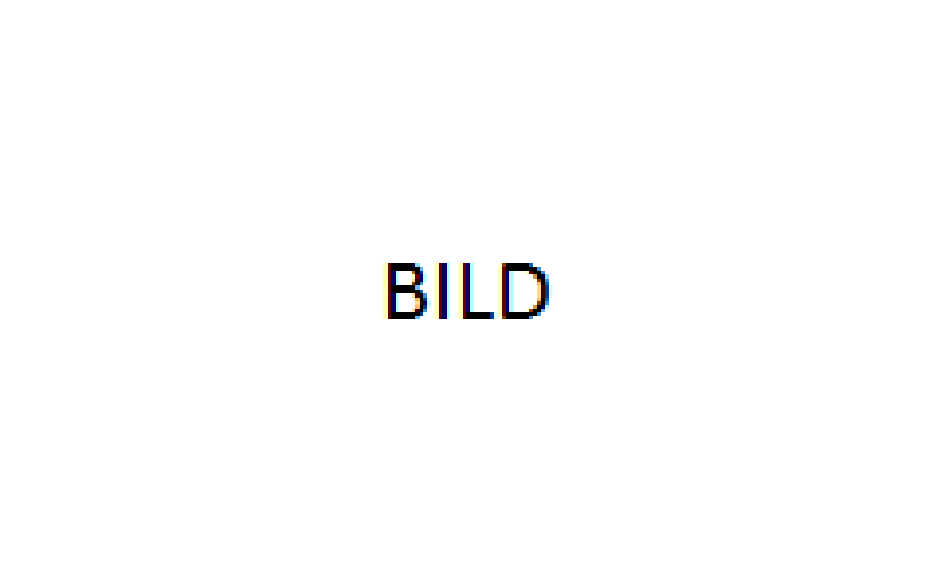
\includegraphics[width=\textwidth]{images/dummy.png}}
        \centering
        \caption{Layout des Editors}
        \label{pic:layout_editor}
\end{figure}
\end{description}

%%%%%%%%%%%%%%%%%%%%%%%%%%%%%%%%%%%%%%%%%%%%%%%%%%%%%%
\subsubsection{Bedienung}
\label{subsubsec04:editor_bedienung}

\begin{description}
\item[Einzelne Veränderungen] \hfill\\
Wie im Abschnitt~\ref{subsubsec04:editor_moegliche_aenderungen}, am Beispiel der Erstellung einer neuen Spalte, fest zu stellen ist, sind Kombinationen von Veränderungen Auslöser für Fehler. So ist das Hinzufügen von neuen Spalten kein Problem, im Gegensatz zum Hinzufügen einer neuen Spalte die ein \texttt{NOT NULL}-Constraint besitzt. \\
Desweiteren ist bei einer Kette von Veränderung nicht immer feststellbar wie die Ursprungstabelle zu der Zieltabelle entwickelt wurde, wenn man die Zwischentabellen nicht kennt.
Zur genaueren Erläuterung betrachte man folgende Grafik:~\ref{pic:table_chain_changes_example}. 

\begin{figure}[ht]
    \frame{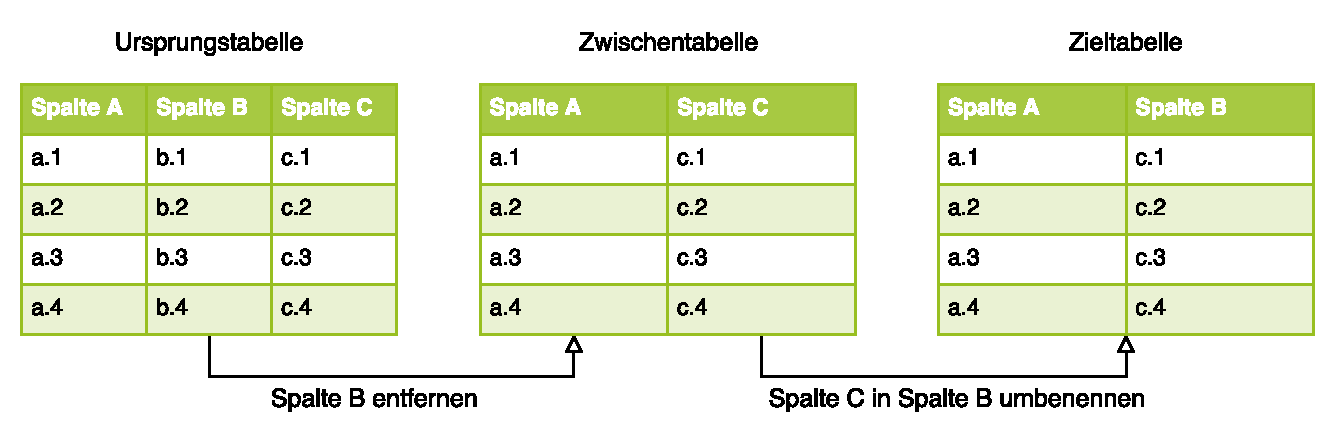
\includegraphics[width=\textwidth]{images/kap-4-chain-changes-ex.pdf}}
        \centering
        \caption{Exemplarische Veränderung einer Tabelle}
        \label{pic:table_chain_changes_example}
\end{figure}

Ohne Betrachtung der Werte und der Zwischentabelle, könnte davon ausgegangen werden, dass nur die Spalte C gelöscht wurde.
Aus diesen Gründen ist es sinnvoll, jeden Schritt im einzelnen zu betrachten und abzuspeichern, an stelle nur der Zieltabelle.
Zusätzlich bietet dies die Möglichkeit dem Benutzer genau mitzuteilen welche Veränderung fehlgeschlagen ist.


\item[Vorschau] \hfill\\
Der Editor zeigt nur die Informationen der Tabelle an. Zum leichteren Verstädnis was die einzelnen Veränderungen bewirken, auf Hinsicht der Tabelle und die Daten, wurde eine Vorschau eingebaut. Die Vorschau zeigt die Tabelle in der typischen tabellarischen Darstellung an, mit ein paar Beispieldaten aus der Tabelle.\\
Eine solche Darstellung wurde schon in der Darstellung der Tabelleninhalte~\ref{subsubsec04:table_content} entwickelt. Diese wurde in einer eigenen Angular 2 Component geschrieben. Dadurch wurde sich die wiederverwendbarkeit von Components benutzt, und kann direkt in Component des Editors mit eingebunden. Damit die Veränderung der Tabelle auch gleichzeitig in beiden Components sichtbar sind, wird das Object der Tabelle in einem Service gespeichert auf das beide Components zugreifen können. In der Grafik~\ref{pic:angular2_architecture} wurde die allgemeine Architektur dargestellt. In der folgenden Grafik wird der Aufbau zwischen dem Service, der Vorschau und des Editors illustriert. \todo[color=green!40]{Bild hinzufügen}%

\begin{figure}[ht]
    \frame{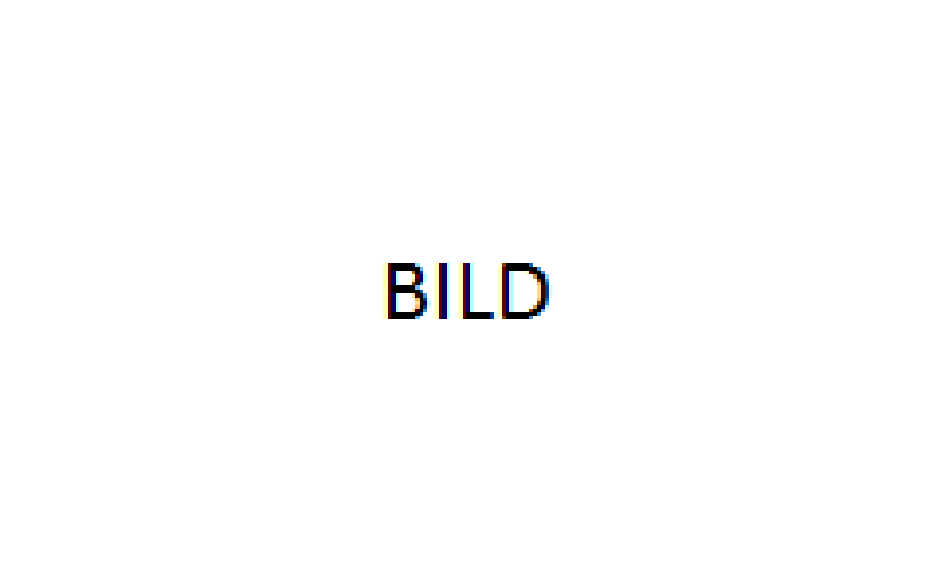
\includegraphics[width=\textwidth]{images/dummy.png}}
        \centering
        \caption{Aufbau des Editors in Angular 2}
        \label{pic:architecture_editor_vorschau}
\end{figure}

Damit die Vorschau noch übersichtlicher wird, werden die einzelnen Spalten farblich gekennzeichnet:
\begin{itemize}
    \item Rot - Spalte wurde gelöscht
    \item Grün - Spalte wurde neu hinzugefügt
    \item Gelb - Spalte wurde verändert
\end{itemize}

\item[Drag \& Drop] \hfill\\
\todo[inline]{Absatz je nach Drag and Drop Status}

\item[Undo \& Redo] \hfill\\
Typescirpt unterstützt unteranderem das Objekt Orientierte Paradigma, damit kann man auf bereits bekannte Entwurfsmuster der Objekt Orientierten Sprachen zurückgegreifen. 
Um eine ``Undo \& Redo'' Funktion einzubauen wurde das Verhaltensmuster ``Command''\footnote{Kommando oder auch Befehl} verwendet.(Mehr dazu:~\ref{subsubsec04:cmd_pattern})

\item[Stack] \hfill\\
Beim Verwenden von ``Undo \& Redo'' und das dabei eingesetzte Entwurfsmuster Kommando können sind die einzelnen Objekte in einer Liste abgelegt(siehe Kapitel:~\ref{subsubsec04:cmd_pattern}).
Durch die Erweiterung der einzelnen Klassen mit einer Funktion die eine String-Repräsentation des Objekts liefern, wird das Erstellen eines Stacks (siehe Grafik:~\ref{pic:stack}) möglich. Dieser zeigt die einzelnen Schritte an, welche bereits gemacht wurden. Mit einem Pfeil wird dargestellt an welcher Stelle im Stack man sich zurzeit befindet. Eine zusätzliche eingebaute Funktion, ist die Möglichkeit durch einen Klick an eine bestimmte Stelle im Stack zu springen. Dabei wird die Undo oder Redo Funktion mehrmals hintereinander ausgeführt, bis die Zielstelle im Stack erreicht ist. Wenn man sich nicht am Ende des Stacks befindet, werden alle Elemente vom Stackpointer bis zum Ende gelöscht, bevor ein neues Element hinzugefügt wird. 

\begin{figure}[ht]
    \frame{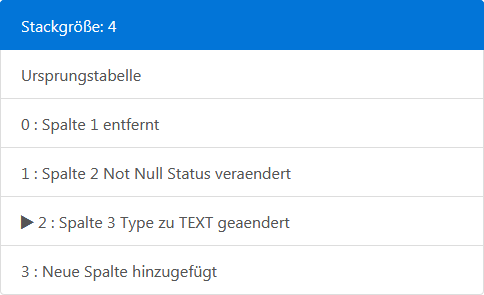
\includegraphics[width=0.7\textwidth]{images/kap-4-stack.png}}
        \centering
        \caption{Stack Beispiel}
        \label{pic:stack}
\end{figure}
\end{description}

Der Stack wird zusätzlich verwendet, um bei aufgetrettenen Fehler darzustellen, welcher Schritt fehlgeschlagen ist. In diesem Fall wird der Eintrag im Stack, rot markiert.


%%%%%%%%%%%%%%%%%%%%%%%%%%%%%%%%%%%%%%%%%%%%%%%%%%%%%%
\subsubsection{Command Pattern}
\label{subsubsec04:cmd_pattern}

\begin{description}
\item[Allgemein] \hfill\\
\item[Arten hier verwendet] \hfill\\
\item[Genereller Aufbau] \hfill\\
\item[Konvertierung Interfaces] \hfill\\
\end{description}

%%%%%%%%%%%%%%%%%%%%%%%%%%%%%%%%%%%%%%%%%%%%%%%%%%%%%%
\subsubsection{Kommunikation mit dem Server}
\label{subsubsec04:kommunikation_cs}
In diesem Abschnitt wird die Kommunikation beschrieben, wie der Client Anfragen an den Server verschickt und welche Antwort erwartet wird.
Die Serverseitige Kommunikation wird im Kapitel:~\ref{subsubsec04:sinatra_client_reaction} beschrieben.

Für alle Anfragen braucht der Server einen Identifikator, der das Projekt definiert und den Namen der Datenbank. Die Anfragen werden per \texttt{HTTP}-Befehle an den Server geleitet.\footnote{Genaueres siehe: TODO Marcus Thesis}\todo{Thesis von Marcus verlinken}%

\begin{description}
\item[Tabelleninhalte vom Server beantragen] \hfill\\
Für die Anfrage der Daten einer Tabelle wird der Tabellenname benötigt. Hinzu kommt, dass in der Ansicht der Daten, durch das Pagening (siehe Kapitel:~\ref{subsubsec04:anz_schema}), dem Server mitgeteilt werden muss, wieviele und ab welchen Tabelleneintrag die Daten erwartet werden.

Als Antwort ist ein 2-Dimensionales Array zu erwarten, welches die Spalten und all deren Zeilen enthält.

\item[Neue Tabellen erstellen] \hfill\\
Für das Erstellen neuer Tabellen muss in dem \texttt{Body} des \texttt{HTTP}-Befehles ein \texttt{JSON}-Objekt sich befinden, welches die zu erstellende Tabelle mit allen Informationen repräsentiert.

Als Antwort erhält der Client das neue komplette Schema zurückgeschickt. Damit kann der Client das Schema aktualisieren.
Dies erhöht den Datentransfer zwischen Server und Client. Eine andere Möglichkeit wäre, den Client das Schema mit dem vorhandenen Objekt selbst zu erweitern. Dies verringert den Datentransfer, kann aber bei Kommunikationsfehlern zu nicht synchronisierten Zuständen führen. Um den gegen zu wirken, wird der Zustand des Server als richtig angenommen und an den Client verschickt.

\item[Tabellen löschen] \hfill\\
In diesen Fall wird nur der Name der Tabelle verschickt. 

Die Antwort ist wieder das komplette aktualisierte Schema.

\item[Tabellen verändern] \hfill\\
In dem \texttt{Body} der Anfrage, ist eine Liste an einzelnen Befehlen~\ref{subsubsec04:cmd_pattern} die an einer Tabelle ausgeführt werden sollen.

Die Antwort, sollten keine Probleme auftretten, ist das aktualisierte Schema.

\item[Fehler beim Ausführen der Befehle] \hfill\\
Beim Erstellen, Löschen und Verändern wird die von der Datenbank mitgeteilt Fehlernachricht an den Client versendet.
Dies können Fehler sein, wie das Erstellen einer Tabelle mit einem Bereits vergebenen Namen oder auch Konsistenzverstöße des Schemas.

Beim Editieren einer Tabelle, wird zusätzlich der genaue Schritt mitgeteilt an welchen ein Fehler aufgetretten ist. Dies wird, wie im Abschnitt~\ref{subsubsec04:editor_bedienung} verwendet um den Fehler im Stack darzustellen.
\end{description}


%%%%%%%%%%%%%%%%%%%%%%%%%%%%%%%%%%%%%%%%%%%%%%%%%%%%%%
\subsubsection{Problematiken}
\label{subsubsec04:problematik}

Während der Entwicklung des Clients kamen einige Probleme auf, die auf mehrere Weisen gelöscht werden könnte. In diesem Abschnitt soll besprochen werden, welche Probleme aufkamen mit den möglichen Lösungen und einer Begründung warum die jeweilige Lösung gewählt wurde.

\begin{description}
\item[Multiple Tabellen simultan verändern] \hfill\\
Jede Veränderung einer Tabelle wird erst übernommen, wenn ein Speicher-Button gedrückt wird. Damit kam die Frage auf, wie damit umgegangen werden soll, wenn man während der Bearbeitung einer Tabelle, denn Editiervorgang verlässt und eine andere Tabelle bearbeitet.
Damit wäre es möglich zwei Tabellen simultan zu verändern. \\
Dies bietet eine vielzahl an möglichen Problemen, die nur schwer vorhersehbar sind. Zusätzlich wäre eine sehr klare und detalierte Kommunikation notwendig bei der Benutzung der Software. Sollte ein Benutzer eine Änderung an einer Tabelle gemacht haben und den Editorvorgang verlassen haben, muss zu jedem Zeitpunkt bestimmt werden, hat der Benutzer den Editiervorgang verlassen, um eine andere Änderung durchzuführen oder weil er den Vorgangh abbrechen will. In Anbetracht der unvorhersehbaren Probleme, ist der Gewinn einer solchen Funktionalität recht gering. Zusätzlich sollte Einsteigern im Thema Datenbanken verständlich gemacht werden, dass die Migration von Datenbanken sich immer nur auf das Nötigste beziehen sollten mit so wenig und kleinen Veränderungen wie möglich. Gerade bei den ersten Projekten, die keinen großen Umfang aufweisen, sollte eine Migration durch gute Vorausplanung verhindert werden. \\
Somit ist es nicht möglich mehrere Tabellen gleichzeitig zu verändern. Da aber während einer Veränderung, der Wunsch bestehen könnte sich die anderen Tabellen anzusehen ohne das der Stack\footnote{die bereits durchgeführt, aber noch nicht gepsiecherten Veränderungen} gelöscht wird, besteht die Möglichkeit den Editiermodus zu verlassen, dass Schema zu betrachten und den Editiervorgang fortsetzen. Beim Betretten eines Editiermodus einer anderen Tabelle, wird der Benutzer dann gegebenenfalls darauf aufmerksam gemacht, dass das Betretten eines anderen Editiervorgangs, den bereits vorhandenen Stack löscht.

\item[Undo vs. selbst verändern] \hfill\\
Die Undo \& Redo Funktion (siehe Kapitel:~\ref{subsubsec04:editor_bedienung}) wurde eingebaut, um eine Erleichterung für den Nutzer zu sein, eine falsche Aktion wieder Rückgängig zu machen. Der durch die Undo \& Redo Funktion entstandene Stack wird auch genutzt, um diesen zum Server zu schicken. \\
Neben der Benutzung von Undo ist es auch möglich die Änderung selbst Rückgängig zu machen. Als Beispiel wäre das Hinzufügen eines \texttt{NOT NULL} Constraint, und dieses wieder manuell zu entnehmen im Gegensatz zur Benutzung der Undo-Funktion. 
Dies würde zu zwei verschiedenen Stacks führen, die auch anders auf Serverseite durchgeführt werden würden. (Siehe Grafik:~\ref{fig:self_vs_undo})\todo[color=green!40]{Bilder gleiche höhe}%

\begin{figure}[h]
  \begin{subfigure}[b]{0.45\textwidth}
    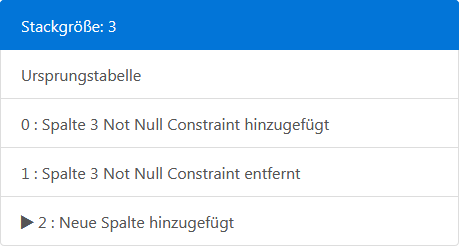
\includegraphics[width=\textwidth]{images/kap-4-self_stack_change.png}
    \caption{Manuell Rückgängig}
    \label{fig:stack_self}
  \end{subfigure}\hfill
  \begin{subfigure}[b]{0.45\textwidth}
    \includegraphics[width=\textwidth]{images/kap-4-undo_stack_change.png}
    \caption{Nutzung von Undo}
    \label{fig:stack_undo}
  \end{subfigure}
  \caption{Vergleich manuell Rückgängig vs. Undo}
  \label{fig:self_vs_undo}
\end{figure}

Dadurch könnten Fehler auftretten, wenn Änderungen auf dem Server durchgeführt werden, von denen der Benutzer ausging sie wurden Rückgängig gemacht. Eine mögliche Lösung des Probelms ist die ``Stack Optimierung'' die im nächsten Abschnitt besprochen wird, warum diese nicht vom Vorteil ist. \\
Bei einigen Änderungen kann man die Absicht des Benutzers nicht abschätzen, und verhindert gegebenenfalls Änderungen die vom Benutzer gewollt sind. Mit der Anzeige des Stacks soll dem Benutzer auch anzeigen, welcher Schritte durchgeführt werden.
Dies ist ein Thema, welches in weiter Entwicklung der Software beachtet werden soll. Mögliche Lösungen können sich ergeben nach Absprache mit Benutzern. 

\item[Stack Optimierung] \hfill\\
Stack Optimierung ist die Verallgemeinerung des Problems ``Undo vs. selbst verändern''. Es gibt viele Ketten an Veränderungen die zusammengefügt oder optimiert werden könnten. Einige Beispiele wären:
\begin{itemize}
    \item Veränderungen einer Spalte die danach gelöscht wird
    \item Manuelles rückgängig machen von Veränderungen
    \item Eine Spalte mehrmals Umbenennen
\end{itemize}

Die jeweiligen Lösungen dafür wären:
\begin{itemize}
    \item Veränderungen nicht durchführen, Spalte sofort löschen
    \item Änderung garnicht erst durchführen
    \item Spalte direkt auf den letzten Namen ändern
\end{itemize}

Alle diese Änderungen könnten aber von dem Benutzer genau in dieser Weise gewollt sein. So könnte ein mehrfaches Umbenennen einer Spalte die Folge sein, wenn bei zwei Spalten die Namen vertauscht werden sollen und dafür der Spaltenname einer Spalte einen temporären Namen erhielt. \\
Sollte eine Optimierung des Stacks dynamisch schon während der Bearbeitung der Tabelle stattfinden, könnte dies zur Verwirrung des Benutzers führen, wenn einzelne Schritte aus dem Stack verschwinden und dann auch nicht mehr per Undo erreicht werden können.
Wenn die Optimierung nach dem Speichern angewendet wird, ist die Benachrichtigung während welchen Schrittes ein Fehler aufkam deutlich erschwert. \\
Die letzten beiden Punkte sind in Anbetracht des ersten Punktes, der Vorhersage was vom Benutzer wirklich gewollt ist, einfacher zu Lösen und weisen trotzdem einen hohen Aufwandswert auf, für den dafür gewonnen Nutzen. \\
Dieses Thema ist eine Optimierung die zu keiner besseren Benutzung der Software selbst führt und der Optimierungsgrad ist relativ gering im Vergleich zum Arbeitsaufwand, und wurde aus diesen Gründen in dieser Arbeits nicht weiter bearbeitet. In der weiteren Entwicklung der Software, kann dieses Thema ein Ansatzpunkt sein. 
\end{description}




\newpage
\subsection{Server}
\label{subsec04:server}
\todo{Einleitungssatz}%

\subsubsection{Sinatra reagieren auf Anfragen}
\label{subsubsec04:sinatra_client_reaction}
In Sinatra werden die Anfragen durch ein \texttt{REST}-ähnliches System angesprochen. Für die Darstellung wird das Datenbankschema benötigt. Dies war bereits integriert und musste nur erweitert werden, um die Information der Foreign Keys(siehe Kapitel:~\ref{subsubsec04:fk_table_server}). \\
Für die jeweiligen Anfragen wurden URLs bestimmt, mit denen die einzelnen Funktionen von Clients angesteuert werden konnte.
Die möglichen Anfragen an den Server sind:
\begin{itemize}
    \item Einen Satz von Daten einer Tabelle
    \item Die Anzahl von vorhandenen Daten in einer Tabelle
    \item Anlegen eienr neuen Tabelle
    \item Löschen einer Tabelle
    \item Editieren einer Tabelle
\end{itemize}

Dabei wurde zur Vorbeugung von ``SQL-Injections''\footnote{\url{https://de.wikipedia.org/wiki/SQL-Injection}} darauf geachtet zu prüfen, ob eine Tabelle zu der Informationen oder Änderungen angefragt wurden, auch wirklich besteht.

\subsubsection{Foreign Keys der Tabellen}
\label{subsubsec04:fk_table_server}
Das Schema wurde bereits an den Client versendet. Um die Foreign Keys dem Schema anzuhängen, wurde zuerst die Struktur der Foreign Keys bestimmt. \\
Die Informationen von Foreign Keys einer Tabelle kann man mit der Verwendung von \texttt{PRAGMAS} erhalten.
\texttt{PRAGMA}-Statement ist eine SQL Erweiterung in SQLite, diese wird für die modifizierung der SQLite Operationen und zum erhalt von internen (nicht tabellen) Informationen.\cite{sqlite_pragma} \\

Die Ausgabe des \texttt{PRAGMA} ``foreign\_key\_list''\footnote{\url{https://sqlite.org/pragma.html\#pragma_foreign_key_list}} enthält die nötigen Informationen. Sie bietet eine Liste einer Liste von zusammengesten Foreign Keys. Diese werden unter anderem durch drei Eigenschaften dargestellt:
\begin{itemize}
    \item den Spaltennamen der Tabelle die ein Foreign Keys Constraint besitzt
    \item auf welche Tabelle dieser Foreign Keys verweist
    \item zu welcher Spalte dieser Tabelle genau verwiesen wird
\end{itemize}

Foreign Keys auf Spalteneben zu speichern erschien somit nicht sinnvoll. Durch die Ausgabe des \texttt{PRAGMA} und das Foreign Keys zusammengesetzt aus mehreren Foreign Keys sein können, werden die Informationen zu Foreign Keys auf Tabellenebene gespeichert. \\
Diese werden mit Anlehnung an die Ausgabe des \texttt{PRAGMA} gespeichert. Es wird eine Liste einer Liste zusammengesetzter Foreign Keys gespeichert, die die drei Information direkt aus dem \texttt{PRAGMA} speicher. \\
Dies wird dann zusammen mit dem bereits versendeten Schema an den Client geliefert.   

\subsubsection{Typsicherung der Tabellenspalten}
\label{subsubsec04:typsicherung}
Die dynamische Typsierung von Spalten ist in SQLite eine Ausnahme verglichen mit anderen Datenbanken, wie schon im Kapitel:~\ref{subsubsec03:zu_entwickeln-Datentypen} geschrieben wurde. \\
Aus diesem Grund wurde dafür gesorgt, dass die Typen in Blattwekzeug sich ähnlicher zum Standart vom SQL verhalten. Dafür müssen die Werte die in eine Tabelle eingetragen werden je nach Typ überprüft werden.
SQLite besitzt drei Möglichkeiten Werte nach einem bestimmten Muster zu prüfen. \\
Der \texttt{LIKE}-Operator ist eine Möglichkeit
\todo{BLOB und LIKE besprechen}%
 SQLite besitzt einen ``REGEXP''-Operator der prüfen kann, ob ein String\footnote{Zeichenkette} einem Regulären Ausdruck entspricht.
Der ``REGEXP''-Operator ist in SQLite nativ nicht implementiert, um die SQLite Datenbankbibliothek so klein wie möglich zu halten. Somit muss zur Laufzeit eine solche Funktion implemtiert und hinzugefügt werden. \\
Die Schnittstelle von Ruby, in dem der Server geschrieben wurde, besitzt eine ``create\_function''-Funktion, um bei der Verbindung mit einer SQLite Datenbank, eine Funktion zu definieren, die dann verwendet werden kann. Damit wurde eine Funktion definiert für den ``REGEXP''-Operator. Der Quelltext dieser Funktion ist hier~\ref{lst:regexp_impl} dargestellt.

\lstinputlisting[
  language=ruby,
  caption=Implmentierung einer Funktion für den ``REGEXP''-Operator,
  label=lst:regexp_impl,
  float=h,
  numbers=left
]{snippets/regexp_impl.rb} 

Die Funktion überprüft im ersten Schritt, ob der übergebene Wert ein leerer String ist. Dies verhindert, dass \texttt{REGEXP} einen Fehler auslöst, da ein leerer String mit dem übergebenen Muster nicht übereinstimmt. Die Datenbank hat bereits mit dem \texttt{NOT NULL}-Constraint eine Überprüfung, ob ein Wert \texttt{NULL} sein darf oder nicht. Aus diesem Grund werden leere Strings, nicht von der Funktion überprüft. \\
Der Rest der Funktion benutzt die Ruby Implementierung einer \texttt{REGEXP}-Funktion.\footnote{\url{https://ruby-doc.org/core-2.1.1/Regexp.html}}
Nachdem der ``REGEXP''-Operator verwendet werden kann, wird in den bei der Definition einer Spalte die Möglichkeit geboten, ein \texttt{Contraint}\footnote{\url{https://sqlite.org/lang_createtable.html}} zu definieren.
Für jeden der vergesehenen Typen wurde ein \texttt{Contraint} erstellt, mit einer individuellen Fehlermeldung. Die vier Typen sind folgende:
\begin{itemize}
    \item \texttt{TEXT} - Eine Menge an beliebigen Zeichen, dafür ist ein Constraint nicht nötig
    \item \texttt{BOOLEAN} - Der Wert darf nur von Wert von 1 oder 0 annehmen, dies kann mit Vergleichsoperatoren implemtiert werden (siehe)
    \item \texttt{INTEGER} - Eine Vorzeichen gebundene ganze Zahl, dafür wird der ``REGEXP''-Operator verwendet, um sicher zustellen, dass nur Zahlen in dem Wert enthalten sind (siehe)
    \item \texttt{FLOAT} - Eine Vorzeichen gebundene relle Zahl, dafür wird der ``REGEXP''-Operator verwendet, damit auch nur solche Zahlen angenommen werden (siehe)
    \item \texttt{URL} - Ein zusätzlicher Typ, der die Möglichkeit bietet URLs in einer Datenbank zu speichern. (siehe) \todo{URL implmentation snipped hinzufügen}
\end{itemize}  

\subsubsection{Anfragen - Darstellung}
\label{subsubsec04:anfragen_darstellung}

\subsubsection{Anfragen - Editor}
\label{subsubsec04:anfragen_editor}

\subsubsection{Unerwartete Probleme}
\label{subsubsec04:server_problems}